\documentclass[conference]{IEEEtran}

\usepackage{fontspec}
\setmainfont{texgyretermes-regular.otf}[
  BoldFont=texgyretermes-bold.otf,
  ItalicFont=texgyretermes-italic.otf,
  BoldItalicFont=texgyretermes-bolditalic.otf
]
\usepackage{booktabs}
\usepackage{balance}
\usepackage{graphicx}
\usepackage{array}
\usepackage{multirow}
\usepackage{microtype}
\usepackage{tikz}
\usetikzlibrary{arrows.meta,positioning}
\usepackage{url}
\usepackage[hidelinks]{hyperref}

\hypersetup{
  pdftitle={Activation-Confirmed Dual-Channel HIL Fault Injection for Payload-Link Supervision},
  pdfauthor={},
  pdfsubject={},
  pdfkeywords={hardware-in-the-loop, fault injection, embedded systems, payload link, reproducibility}
}

\title{Activation-Confirmed Dual-Channel HIL Fault Injection for Payload-Link Supervision}
\author{}

\begin{document}
\maketitle

\begin{abstract}
Payload communication is an important fault boundary in embedded controllers: a payload can become silent, return a corrupted response, or answer after a deadline. This paper presents an activation-confirmed hardware-in-the-loop (HIL) method that exercises those behaviors on a physical UART link. A host orchestrates a controller board and a commandable payload-simulator board through independent serial-observation channels. A trial is accepted only after payload-side confirmation of both fault activation and NORMAL restoration; controller-side markers then define detection and recovery. The primary campaign comprises two 65-s nominal windows and 90 sequential trials on one board pair, with 30 trials per fault mode. All 90 trials were valid, and the predefined detector and recovery markers were each observed in 30/30 valid trials for every mode. Host-observed command-to-marker medians ranged from 359.5 to 406.0~ms for detection and from 296.5 to 359.0~ms for recovery. A separate F411 extension used the same predefined 12-row protocol on each of two physical pairs; reported separately, both pairs showed clean normal controls, accepted 90-ms responses without fault transitions, and timeout/sequence-rejection/OFFLINE behavior with restoration and recovery at 100 and 110~ms. The contribution is a dual-channel protocol that distinguishes requested, activated, detected, restored, and recovered events, supported by hash-locked empirical records. Results are bounded to the evaluated setups and are not a device-population reliability or controller-internal timing estimate.
\end{abstract}

\begin{IEEEkeywords}
hardware-in-the-loop, fault injection, embedded systems, payload link, reproducibility
\end{IEEEkeywords}

\section{Introduction}

Embedded controllers commonly supervise peripheral or payload communication by checking whether responses arrive, whether their integrity fields are valid, and whether a previously unavailable peer returns to service. Testing only a healthy peer leaves those paths weakly observed. Conversely, an injection campaign can become difficult to interpret when the experiment records only a sent command, mixes controller and injector evidence, or reports host timestamps as if they were internal execution times.

Fault injection has long been used to exercise fault-handling mechanisms under controlled conditions. Arlat \emph{et al.} characterize an experiment through faults, activations, readouts, and measures (the FARM sets)~\cite{arlat1990}. HIL studies place real controller hardware against a controllable environment and inject abnormal signals without modifying the system under test~\cite{abboush2022,abboush2024}. Nanosatellite research has also injected faults into a payload communication bus and reused modeled interoperability tests with physical subsystems~\cite{batista2019,conceicao2025}. These principles motivate a focused experiment at a payload communication endpoint.

This paper evaluates one physical controller/payload-simulator pair. The simulator exposes three commandable behaviors: silence, CRC corruption, and response delay. A host harness confirms the selected behavior on the simulator channel before accepting a controller-side detection event. After a fixed observation interval, the harness restores normal behavior, confirms that restoration, and observes a predefined recovery marker. Every raw serial record retains a host timestamp, exact bytes, and readable rendering. The resulting claim scope is locked before manuscript assembly: quantitative statements are projected from hash-verified frozen summaries, and unsupported extrapolations are excluded.

The paper makes three bounded contributions:

\begin{itemize}
  \item an activation-confirmed dual-channel HIL procedure that separates requested, activated, detected, restored, and recovered events;
  \item a descriptive evaluation of nominal behavior, predefined detection/recovery outcomes, host-observed command-to-marker latency, and pair-specific protocol-level reproduction on two separate F411 configurations; and
  \item an evidence-locking workflow that connects manuscript tables to immutable experiment summaries and validation artifacts.
\end{itemize}

The study does not compare against a C0 ablation, treat sequential trials as independent hardware replicas, or infer controller-internal timing. These boundaries are central to the interpretation rather than post-hoc qualifications.

\begin{figure*}[t]
\centering
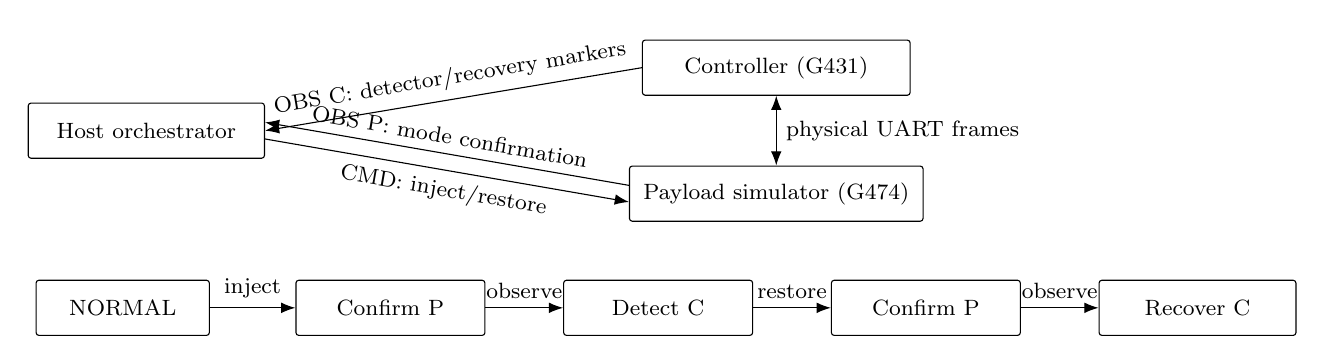
\begin{tikzpicture}[
  font=\footnotesize,
  box/.style={draw,rounded corners=1pt,align=center,minimum height=7mm,inner xsep=5pt},
  flow/.style={-{Latex[length=1.8mm]},line width=0.4pt},
  bi/.style={{Latex[length=1.8mm]}-{Latex[length=1.8mm]},line width=0.4pt}
]
\node[box,minimum width=30mm] (host) at (0,0) {Host orchestrator};
\node[box,minimum width=34mm] (ctrl) at (8.0,0.8) {Controller (G431)};
\node[box,minimum width=34mm] (payload) at (8.0,-0.8) {Payload simulator (G474)};
\draw[flow] (ctrl.west) -- node[above,sloped]{OBS C: detector/recovery markers} (host.east);
\draw[flow] ([yshift=-3pt]host.east) -- node[below,sloped]{CMD: inject/restore} ([yshift=-3pt]payload.west);
\draw[flow] ([yshift=3pt]payload.west) -- node[above,sloped]{OBS P: mode confirmation} ([yshift=3pt]host.east);
\draw[bi] (ctrl.south) -- node[right]{physical UART frames} (payload.north);

\node[box,minimum width=22mm] (n0) at (-0.3,-2.25) {NORMAL};
\node[box,minimum width=24mm] (act) at (3.1,-2.25) {Confirm P};
\node[box,minimum width=24mm] (det) at (6.5,-2.25) {Detect C};
\node[box,minimum width=24mm] (rst) at (9.9,-2.25) {Confirm P};
\node[box,minimum width=25mm] (rec) at (13.35,-2.25) {Recover C};
\draw[flow] (n0) -- node[above]{inject} (act);
\draw[flow] (act) -- node[above]{observe} (det);
\draw[flow] (det) -- node[above]{restore} (rst);
\draw[flow] (rst) -- node[above]{observe} (rec);
\end{tikzpicture}
\caption{Dual-channel setup and accepted trial sequence. OBS C and OBS P are independent host serial channels; payload confirmation gates scoring after injection and restoration.}
\label{fig:protocol}
\end{figure*}

\section{Related Work}

The FARM formulation separates the injected fault, its activation, system readouts, and resulting measures~\cite{arlat1990}. This separation is important when a command to an injector may not prove that the requested behavior became active. Experimental conclusions also depend on the chosen fault model and observation boundary~\cite{piper2015}. In this study, the commanded payload behavior is the fault, payload-side mode confirmation is activation evidence, controller markers are readouts, and observed counts plus host-timestamp distributions are measures.

Recent automotive HIL frameworks combine a real controller with a simulated environment and programmatic signal faults. Abboush \emph{et al.} first demonstrated real-time sensor/actuator fault injection around an ECU prototype~\cite{abboush2022}, then extended the approach into a virtual testing framework for single and simultaneous faults in varied driving scenarios~\cite{abboush2024}. Those studies emphasize real-time dynamic-system validation. The present work instead targets a framed serial endpoint and the evidentiary sequence from a fault request through confirmed activation and restoration to controller detection and recovery.

Closest to the application boundary here, Batista \emph{et al.} place a failure-emulator mechanism in the NanosatC-BR2 payload I$^2$C channel and exercise robustness tests in MIL and HIL configurations~\cite{batista2019}. Concei\c{c}\~ao and Mattiello-Francisco later systematize CubeSat interoperability models, generated test cases, and staged reuse from simulated boards to physical subsystems~\cite{conceicao2025}. These works establish communication-bus fault injection and systematic interoperability testing; they do not report the specific empirical construct evaluated here: independent host observation of controller and payload endpoints, acceptance gated by explicit activation/restoration confirmations, and byte-preserving per-trial traces. Evidence locking supports reproducibility of that construct but is not claimed as its sole novelty.

\begin{table}[t]
\caption{Selected adjacent HIL evaluation boundaries.}
\label{tab:related}
\centering
\scriptsize
\begin{tabular}{@{}>{\raggedright\arraybackslash}p{1.45cm}>{\raggedright\arraybackslash}p{2.0cm}>{\raggedright\arraybackslash}p{3.65cm}@{}}
\toprule
Study & Boundary & Evaluation emphasis \\
\midrule
Abboush~\cite{abboush2022,abboush2024} & Automotive model signals & Dynamic behavior under programmatic faults \\
Batista~\cite{batista2019} & Nanosatellite I$^2$C bus & Interoperability and robustness requirements \\
Concei\c{c}\~ao~\cite{conceicao2025} & Staged CubeSat MIL/HIL & Model-based interoperability tests \\
This work & UART payload endpoint & Confirmation-gated dual-channel observations \\
\bottomrule
\end{tabular}
\end{table}

\section{System and Research Questions}

\subsection{Payload-Link Supervision}

The setup consists of a NUCLEO-G431RB controller and a NUCLEO-G474RE payload simulator connected by a UART at 115200~8N1 with common ground. The controller periodically exchanges framed messages with the payload. Its observable supervision paths include response timeout, CRC rejection, transition to an offline state, and a later recovery marker. Boot and runtime mechanisms provide architectural context, but the empirical contribution is limited to the payload link.

The payload simulator accepts host commands for NORMAL, SILENT, BAD\_CRC, and DELAYED modes. SILENT withholds a response. BAD\_CRC returns a response with an invalid CRC. DELAYED waits 250~ms before responding, exceeding the inspected 100-ms controller deadline. A second host serial channel captures the simulator's exact mode confirmation. Thus, a sent command alone is insufficient activation evidence.

\subsection{Locked Research Questions}

The study asks only the following descriptive questions:

\begin{description}
  \item[RQ1:] What payload-link status and counter behavior is observed during the predefined pre- and post-campaign nominal (N0) windows?
  \item[RQ2:] For SILENT, BAD\_CRC, and DELAYED, in how many valid sequential trials are activation, the mode-specific detector, NORMAL restoration, and recovery markers observed?
  \item[RQ3:] What are the per-mode distributions of host-observed command-to-detector-marker and restore-command-to-recovery-marker latency?
\end{description}

N0 denotes a healthy nominal condition; it is not a comparative or ablation baseline.

\section{Evaluation Method}

\subsection{Nominal Windows}

A 65-s N0 window was captured before the campaign and another after it. A window was valid if it contained at least 10 controller status records, all records reported ONLINE, the successful-message counter increased strictly, timeout/CRC/sequence/recovery counter deltas were zero, and no prohibited transition, rejection, recovery, or post-start link-start marker appeared.

\subsection{Trial Protocol and Outcomes}

Seed 20260830 fixed the order of 90 sequential trials and their pre-injection offsets: 30 trials for each mode. Every trial used the same physical pair. As Fig.~\ref{fig:protocol} shows, the protocol first commanded NORMAL and observed the precondition, waited the seeded offset, sent the selected mode, and required the matching simulator confirmation. The controller was then observed for 4~s. The harness sent NORMAL, required the simulator's NORMAL confirmation, and observed the controller for a further 3~s.

For SILENT, the predefined detector was the first post-injection timeout or offline marker. For BAD\_CRC, it was the first explicit CRC-rejection marker. For DELAYED, it was the first timeout or offline marker, consistent with the configured delay and inspected deadline. OFFLINE was retained as a secondary observation and was not required for BAD\_CRC detection. Recovery required a controller recovery marker after the restore command and a confirmed NORMAL restoration. A restart field recorded only the presence or absence of a post-injection link-start marker; its absence was not interpreted as independent reset evidence.

A trial was valid only when its invalid-reason field was empty and both activation and restoration were confirmed on the simulator channel. Machine validation cross-checked 90 plan rows, 90 result rows, and all 180 controller/payload raw logs and reported no issues.

\subsection{Measurement and Analysis}

Detection latency is the host timestamp of the first predefined controller detector marker minus the host timestamp at injection-command send. Recovery latency is the host timestamp of the controller recovery marker minus the host timestamp at NORMAL-command send. These intervals include serial transport, USB, driver buffering, host scheduling, and timestamping effects; there was no host/MCU clock synchronization.

Analysis is descriptive. Per mode, we report detection and recovery counts and observed proportions. Latency summaries contain sample count, median, inclusive-linear quartiles, interquartile range (IQR), minimum, and maximum. No confidence interval, hypothesis test, or between-mode ranking is reported. The observations are sequential measurements on one setup, not independent device replicates; device-population uncertainty cannot be estimated from this single board pair.

\subsection{Cross-Configuration Extension}

Two separate F411 controller/payload pairs each executed an identical, predefined 12-row campaign: three normal controls and three observations at each of 90, 100, and 110~ms. Both pairs used the same fixed F411 implementation, firmware hashes, order, four-second exposure, confirmation gates, and validity rules. Each pair is analyzed with its own denominator of three per condition. Rows and counters are not pooled across pairs, and this extension does not compare binary images or timing with the primary G431/G474 setup.

\subsection{Construct Validity and Controls}

The intervention construct is a confirmed endpoint behavior, not merely a host command. The payload channel had to report the requested mode after injection and NORMAL after restoration; otherwise the trial was invalid. This supports temporal attribution within the protocol but does not make silence, CRC corruption, or delay equivalent to an electrical, environmental, or radiation-induced fault. The response construct is likewise operational: detection and recovery mean that the predefined controller marker appeared in the permitted observation phase. They do not expose every internal state transition.

Three controls reduce ambiguity without creating independent replication. First, each trial begins from an observed NORMAL precondition, and fixed fault/recovery windows separate detection from recovery scoring. Second, the seeded order and pre-injection offsets make the executed sequence reproducible while avoiding an unrecorded adaptive order. Third, controller and payload bytes are recorded separately before the result row is validated against both raw logs. These controls strengthen within-setup traceability. They do not remove shared hardware, host, thermal, or state-history conditions, and they cannot support population-level uncertainty estimates.

\begin{table}[t]
\caption{Validated N0 windows. Only within-window deltas are interpreted.}
\label{tab:n0}
\centering
\footnotesize
\begin{tabular}{lrrrrrr}
\toprule
Phase & Status & $ok$ first--last & TO & CRC & SEQ & REC \\
\midrule
Pre  & 13 & 1835--1955 & 0 & 0 & 0 & 0 \\
Post & 13 & 3049--3169 & 0 & 0 & 0 & 0 \\
\bottomrule
\end{tabular}
\end{table}

\section{Results}

\subsection{RQ1: Nominal Behavior}

Both N0 windows were valid. Each lasted 65.0~s and contained 13 ONLINE status records. The successful-message counter increased strictly from 1835 to 1955 before the campaign and from 3049 to 3169 after it. Within both windows, timeout, CRC, sequence, and recovery counter deltas were zero, and the prohibited-marker list was empty (Table~\ref{tab:n0}). The different absolute counter levels reflect preceding activity; only within-window changes are evaluated.

\subsection{RQ2: Predefined Outcomes}

All 90 planned trials were retained as valid. Each mode had 30 confirmed activations and 30 confirmed NORMAL restorations. The predefined detector and recovery markers were each observed in 30/30 valid trials per mode (observed proportion 1.0). OFFLINE was observed in 30/30 trials for each mode during the configured fault window, including BAD\_CRC, where it was not the detection criterion. No post-injection link-start marker was recorded (Table~\ref{tab:outcomes}); this marker absence is not proof that no reset occurred.

The 30/30 values describe the retained sequential observations rather than draws from an identified device population. Their evidentiary role is to show that no valid trial in this campaign lacked the predefined marker. They are not converted into a reliability estimate or a confidence bound because repeated runs on the same hardware do not establish the sampling model required for such a population claim.

\begin{table}[t]
\caption{Observed outcomes by injected mode. Proportions are descriptive observations on one board pair.}
\label{tab:outcomes}
\centering
\footnotesize
\begin{tabular}{lccccc}
\toprule
Mode & Valid & Detect & Recover & Offline & Start \\
\midrule
SILENT   & 30/30 & 30/30 & 30/30 & 30/30 & 0/30 \\
BAD\_CRC  & 30/30 & 30/30 & 30/30 & 30/30 & 0/30 \\
DELAYED  & 30/30 & 30/30 & 30/30 & 30/30 & 0/30 \\
\bottomrule
\end{tabular}
\end{table}

\subsection{RQ3: Host-Observed Latency}

Table~\ref{tab:latency} reports both host-observed intervals. Command-to-detector-marker medians were 383.0~ms for SILENT, 359.5~ms for BAD\_CRC, and 406.0~ms for DELAYED. Restore-command-to-recovery-marker medians were 297.0, 359.0, and 296.5~ms, respectively. The IQRs and full observed ranges show substantial within-mode dispersion. These summaries are not compared inferentially and do not define internal controller execution bounds.

\begin{table}[t]
\caption{Host-observed command-to-marker latency (ms), $n=30$ per row. Quartiles use the frozen inclusive-linear definition.}
\label{tab:latency}
\centering
\scriptsize
\begin{tabular}{@{}llrrrrr@{}}
\toprule
Mode & Int. & Median & Q1 & Q3 & IQR & Min--Max \\
\midrule
SILENT & Det. & 383.0 & 288.75 & 485.0 & 196.25 & 125--578 \\
BAD\_CRC & Det. & 359.5 & 171.25 & 464.25 & 293.0 & 78--531 \\
DELAYED & Det. & 406.0 & 297.0 & 512.0 & 215.0 & 156--610 \\
\midrule
SILENT & Rec. & 297.0 & 144.25 & 375.0 & 230.75 & 78--516 \\
BAD\_CRC & Rec. & 359.0 & 113.75 & 417.25 & 303.5 & 47--531 \\
DELAYED & Rec. & 296.5 & 187.25 & 425.5 & 238.25 & 94--531 \\
\bottomrule
\end{tabular}
\end{table}

\subsection{Cross-Configuration Protocol-Level Reproduction}

Table~\ref{tab:f411} reports the two F411 pairs separately. Each campaign retained 12/12 valid rows. For each pair, all three normal controls had zero adverse markers; all three 90-ms rows accepted delayed responses without timeout, rejection, or OFFLINE; and all three rows at both 100 and 110~ms showed timeout, sequence rejection, and OFFLINE followed by confirmed NORMAL restoration and recovery. Neither 100- nor 110-ms condition accepted a mode-3 response. Thus, under the identical predefined protocol and fixed F411 implementation, the same condition-level supervision pattern was observed on each of two separate physical F411 controller/payload pairs.

\begin{table}[t]
\caption{Separate F411 pair outcomes; each cell retains its own denominator and no cross-pair pooling is performed.}
\label{tab:f411}
\centering
\scriptsize
\begin{tabular}{lccccc}
\toprule
Pair & Valid & NC clean & 90-ms accept & 100-ms F/R & 110-ms F/R \\
\midrule
Pair-1 & 12/12 & 3/3 & 3/3 & 3/3 & 3/3 \\
Pair-2 & 12/12 & 3/3 & 3/3 & 3/3 & 3/3 \\
\bottomrule
\end{tabular}
\end{table}

Here F/R denotes the predefined timeout/sequence-rejection/OFFLINE pattern with restoration and recovery, not a pooled success metric. Post-activation mode-0 accepts were retained as boundary/pipeline observations in four Pair-1 rows and three Pair-2 rows; subsequent markers remained attributable to the planned conditions. In every 100- and 110-ms row, cumulative status-counter deltas (timeout 8 and sequence 8) exceeded the two explicit timeout-transition and one explicit sequence-rejection markers, so these quantities are reported separately.

\section{Discussion and Limitations}

The dual-channel protocol closes a specific evidentiary gap between requesting a behavior and observing that the payload simulator entered it. Within the primary frozen setup, all retained injections produced their predefined controller detector evidence and were followed by a recovery marker after confirmed restoration. The N0 windows provide bounded healthy observations on both sides of that campaign. The separate F411 campaigns add protocol-level physical reproduction across two configurations without changing the one-pair interpretation of the primary results. They do not establish behavior on an unobserved device population, and population-level uncertainty is not estimated from two purposively evaluated pairs.

The experiment has several deliberate limitations. First, the primary 90 trials used one physical board pair and occurred sequentially; each 12-row F411 campaign was likewise sequential within its own pair. Trial outcomes may therefore share device, thermal, state-history, host, and timing conditions. Second, nominal evidence is limited to two 65-s primary windows and one 65-s gate per F411 pair; it does not establish long-duration stability. Third, no fair C0 ablation was constructed, so neither a treatment effect nor comparative superiority is supported. Fourth, timing is based on host command and serial-receipt timestamps. UART, USB, operating-system, and scheduling delays are included, and MCU-internal latency is unknown.

Fifth, outcomes are marker based. A recorded detector or recovery marker supports the corresponding protocol definition but not every internal state transition. Conversely, absence of a link-start marker does not independently prove the controller never reset. Literal heartbeat or watchdog status strings were not treated as independent health measurements. Sixth, only silence, bad CRC, and one delayed-response setting were exercised under fixed observation windows. Other delay magnitudes, corruption patterns, intermittent behavior, concurrent loads, and recovery horizons remain untested.

Finally, no environmental stress was applied: temperature, vibration, electromagnetic conditions, power transients, and radiation were not varied or measured. The evidence therefore provides no environmental robustness, flight-qualification, mission-assurance, or complete-system validation result. Binary-to-readback agreement strengthens provenance for the evaluated firmware, but it does not add trials or broaden the empirical population.

\section{Reproducibility and Evidence Lock}

The campaign package retains a fixed seed and run plan, per-trial result rows, 180 raw serial logs, validation output, descriptive summaries, firmware, and SHA-256 inventories. The raw format records host UTC time, exact received bytes, and escaped text. A separate table generator first verifies the frozen hashes of the campaign summary, campaign validation, and both N0 validations, then deterministically projects the manuscript CSV tables. The generator records its own hash and the input/output hashes.

This mechanism supports inspection of how every number in Tables~\ref{tab:n0}--\ref{tab:latency} reaches the manuscript. A separate provenance-checked generator verifies both F411 source and backup inventories and projects Table~\ref{tab:f411} without pooling. These checks prevent an unnoticed source change from silently producing new tables. Replication beyond the two evaluated F411 pairs remains untested, and anonymous review omits any author-revealing repository location. Artifact access can be provided in a non-identifying form or after review according to venue policy.

\section{Conclusion}

This paper presented activation-confirmed dual-channel HIL fault injection for payload-link supervision using a controller board, a commandable payload-simulator board, and independent host observation channels. Two bounded nominal windows and 90 sequential primary trials provide a traceable description of predefined detection and recovery markers and host-observed command-to-marker latency distributions. Under an identical predefined F411 protocol, the same condition-level supervision pattern was separately observed on each of two physical controller/payload pairs. The methodological result remains setup bounded: confirmed link-endpoint behavior can be connected to controller evidence and immutable logs without converting repeated observations into population, reliability, MCU-equivalence, or internal-timing claims. Future work may expand fault models, observation duration, and independent instrumentation; those extensions are not implied by the present datasets.

\balance
\bibliographystyle{IEEEtran}
\bibliography{references}

\end{document}
